\subsection{Mô hình hoá quy trình nghiệp vụ}

% ---------------------- RENT PROCESS ----------------------
\subsubsection{Quy trình thuê xe (UC-02, UC-03, UC-04)}
\label{subsec:rent-activity}
\small\textit{(Hình \ref{fig:rent-activity})}
\subsubsection*{Mục tiêu:}
Cho phép người dùng tìm kiếm, xem thông tin và đặt thuê xe máy điện trong khu vực mong muốn thông qua ứng dụng.
\subsubsection*{Actor chính: Người thuê (Renter)}
\subsubsection*{Các bước chính:}
1. Người thuê đăng nhập và chọn chức năng “Tìm xe gần tôi” hoặc nhập vị trí thủ công.\newline
2. Hệ thống xác định vị trí, truy vấn và hiển thị danh sách xe khả dụng.\newline
3. Người thuê chọn xe để xem thông tin chi tiết (giá, pin, vị trí, chủ xe, đánh giá).\newline
4. Người thuê chọn “Đặt thuê”, nhập thời gian và xác nhận.\newline
5. Hệ thống gợi ý thời điểm thuê tối ưu (AI), kiểm tra tình trạng xe, tạo đơn thuê và gửi thông báo đến chủ xe.\newline
6. Người thuê nhận xác nhận thành công, hoàn tất quá trình thuê nếu chủ xe xác nhận cho thuê.
\subsubsection*{Luồng thay thế:}
Người dùng có thể nhập vị trí thủ công khi không bật GPS. Nếu không có xe khả dụng, hệ thống gợi ý mở rộng phạm vi hoặc thời gian khác.

% ---------------------- RETURN PROCESS ----------------------
\subsubsection{Quy trình trả xe (UC-05, UC-06, UC-07)}
\label{subsec:return-activity}
\small\textit{(Hình \ref{fig:return-activity})}
\subsubsection*{Mục tiêu:}
Cho phép người thuê kết thúc hành trình, trả xe và thực hiện thanh toán, đồng thời gửi đánh giá cho chủ xe hoặc phương tiện sau khi hoàn tất chuyến đi.
\subsubsection*{Actor chính: Người thuê (Renter)}
\subsubsection*{Các bước chính:}
1. Người thuê chọn chức năng “Trả xe” trong ứng dụng. \newline
2. Hệ thống xác nhận vị trí hiện tại của xe hoặc yêu cầu nhập thủ công nếu không định vị được. \newline
3. Hệ thống tính toán chi phí thuê thực tế dựa trên thời gian và quãng đường. \newline
4. Người thuê xác nhận thanh toán. \newline
5. Sau khi thanh toán thành công, hệ thống cập nhật trạng thái xe thành “Available”. \newline
6. Ứng dụng hiển thị màn hình đánh giá xe và chủ xe. \newline
7. Người thuê gửi đánh giá (số sao, nội dung) để hoàn tất quy trình.
\subsubsection*{Luồng thay thế:}
- Nếu người thuê trả xe sớm hơn thời gian dự kiến, hệ thống tự động điều chỉnh chi phí. \newline
- Nếu GPS không xác định được vị trí, hệ thống yêu cầu người dùng nhập vị trí trả xe thủ công.

\begin{figure}[H]
    \centering
    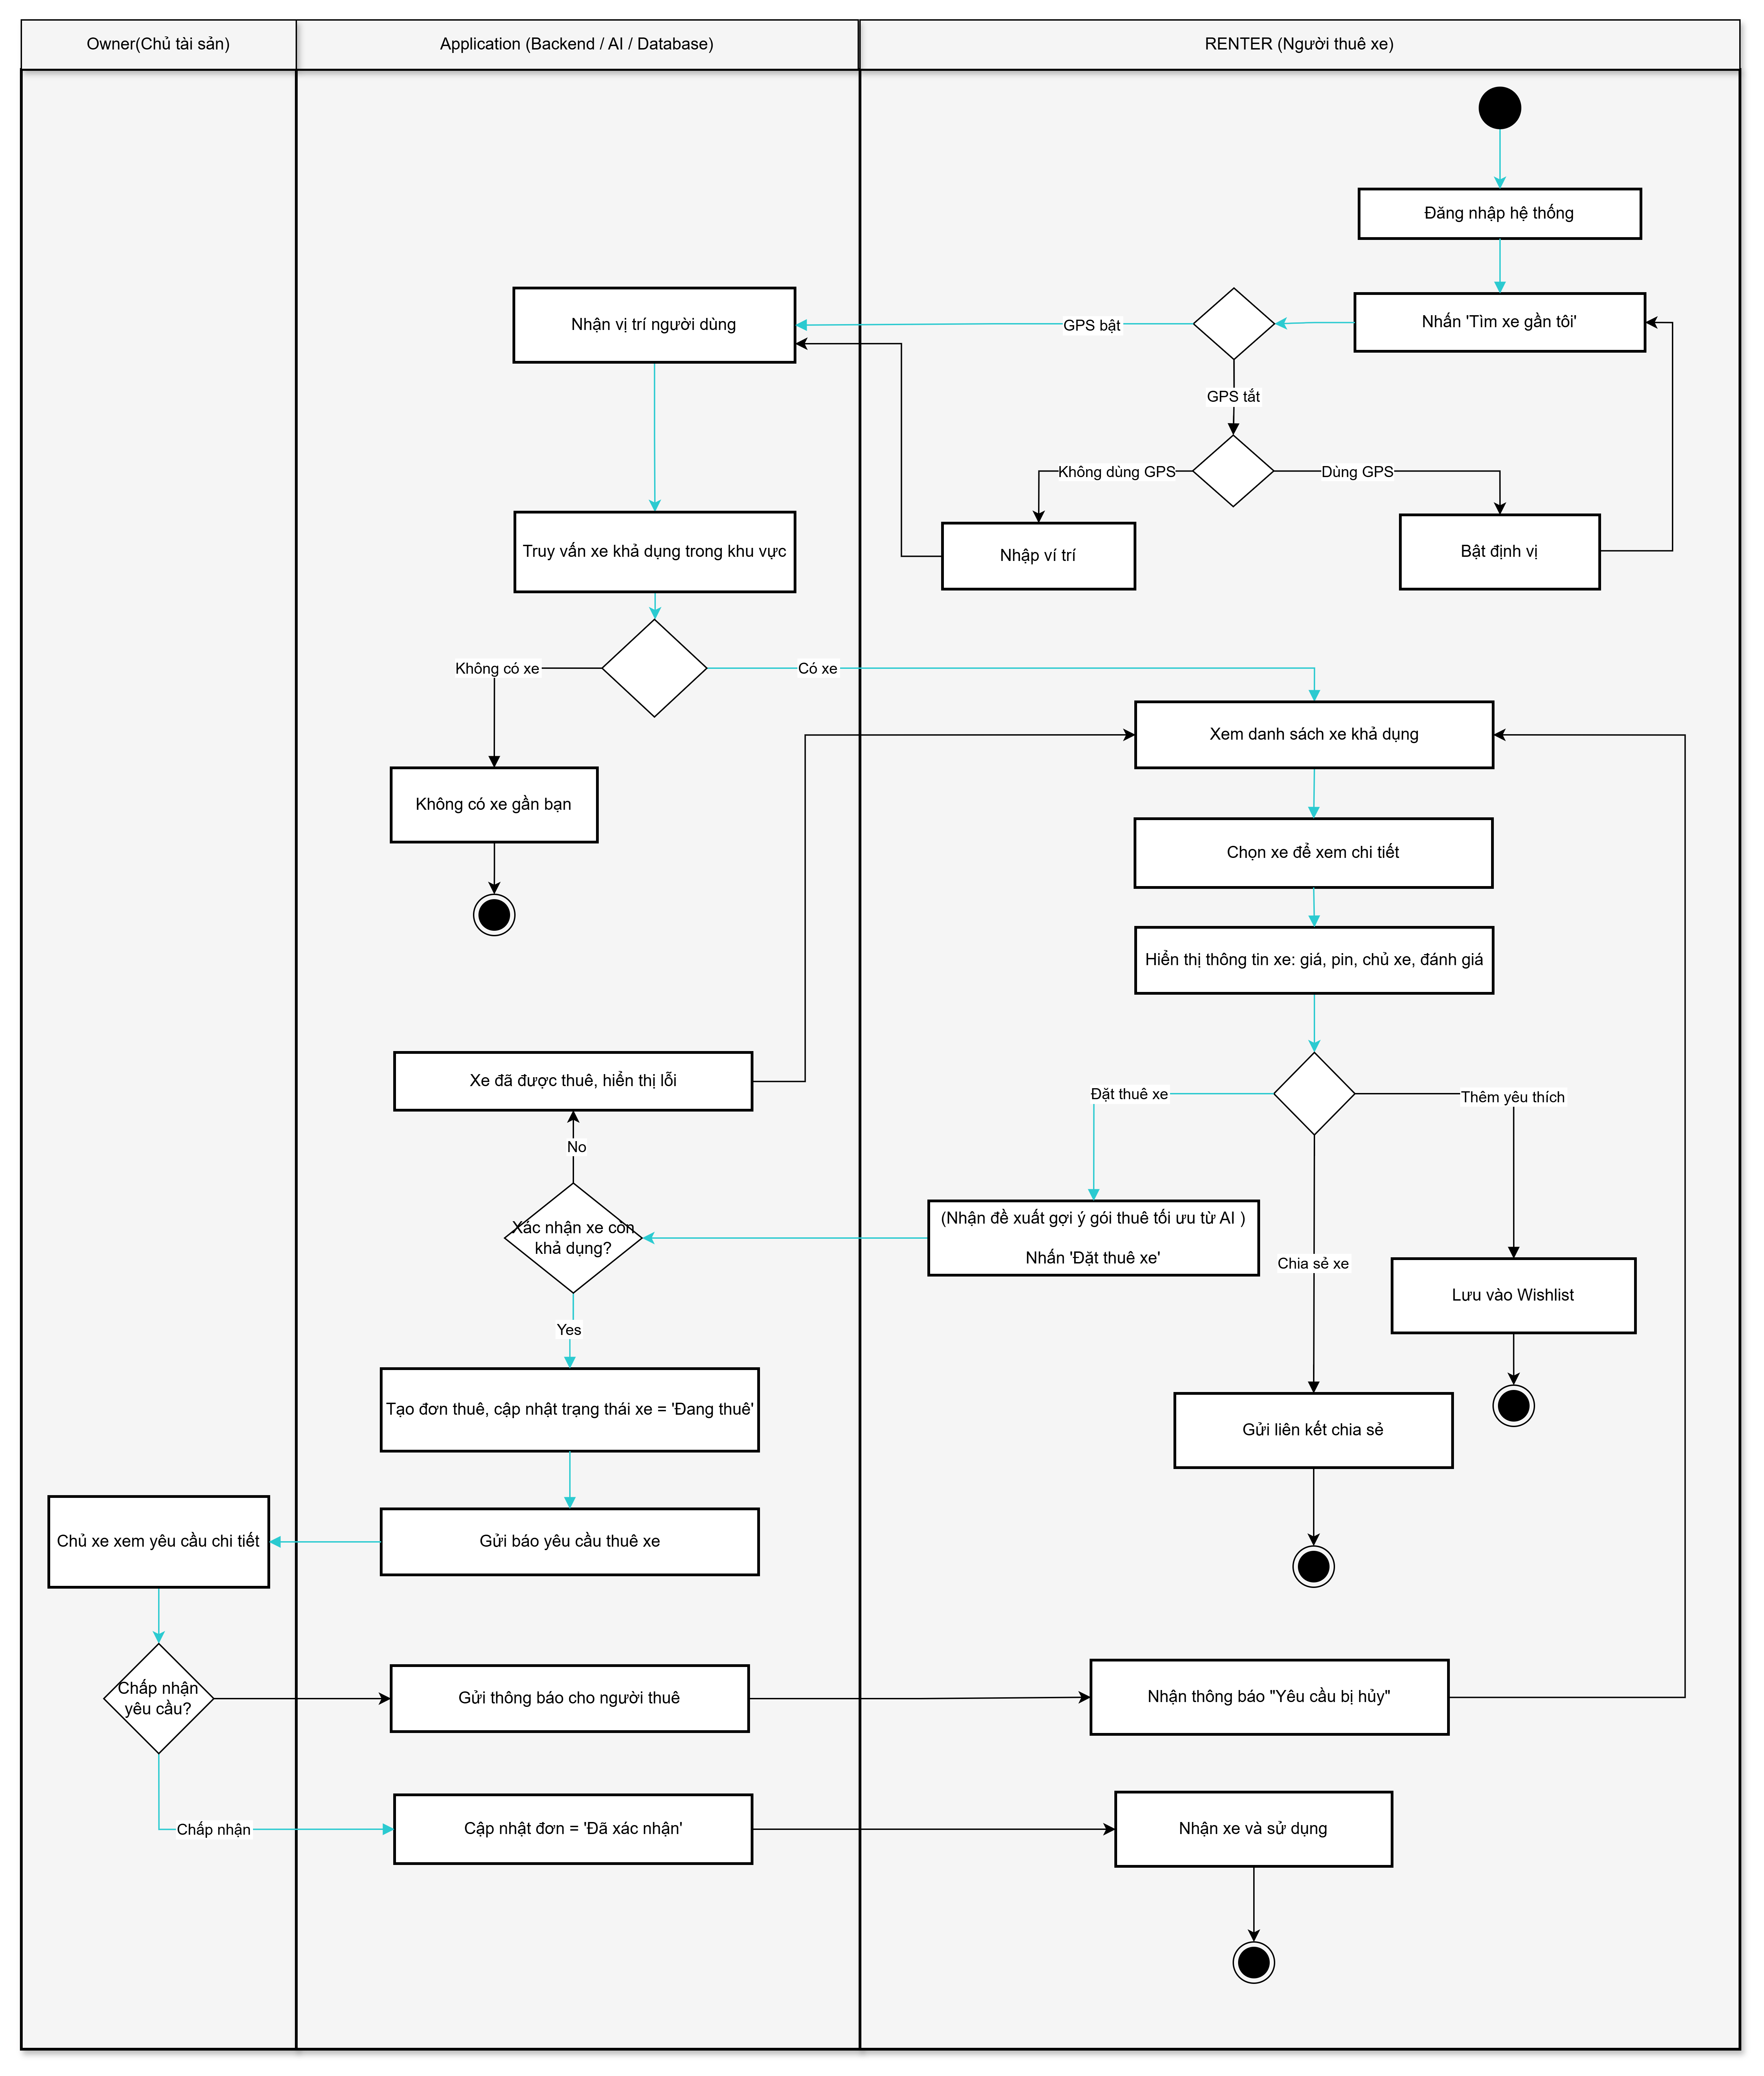
\includegraphics[width=1\textwidth]{Images/Activity/rent.png}
    \caption{Renting Activity Diagram}
    \label{fig:rent-activity}
\end{figure}

\begin{figure}[H]
    \centering
    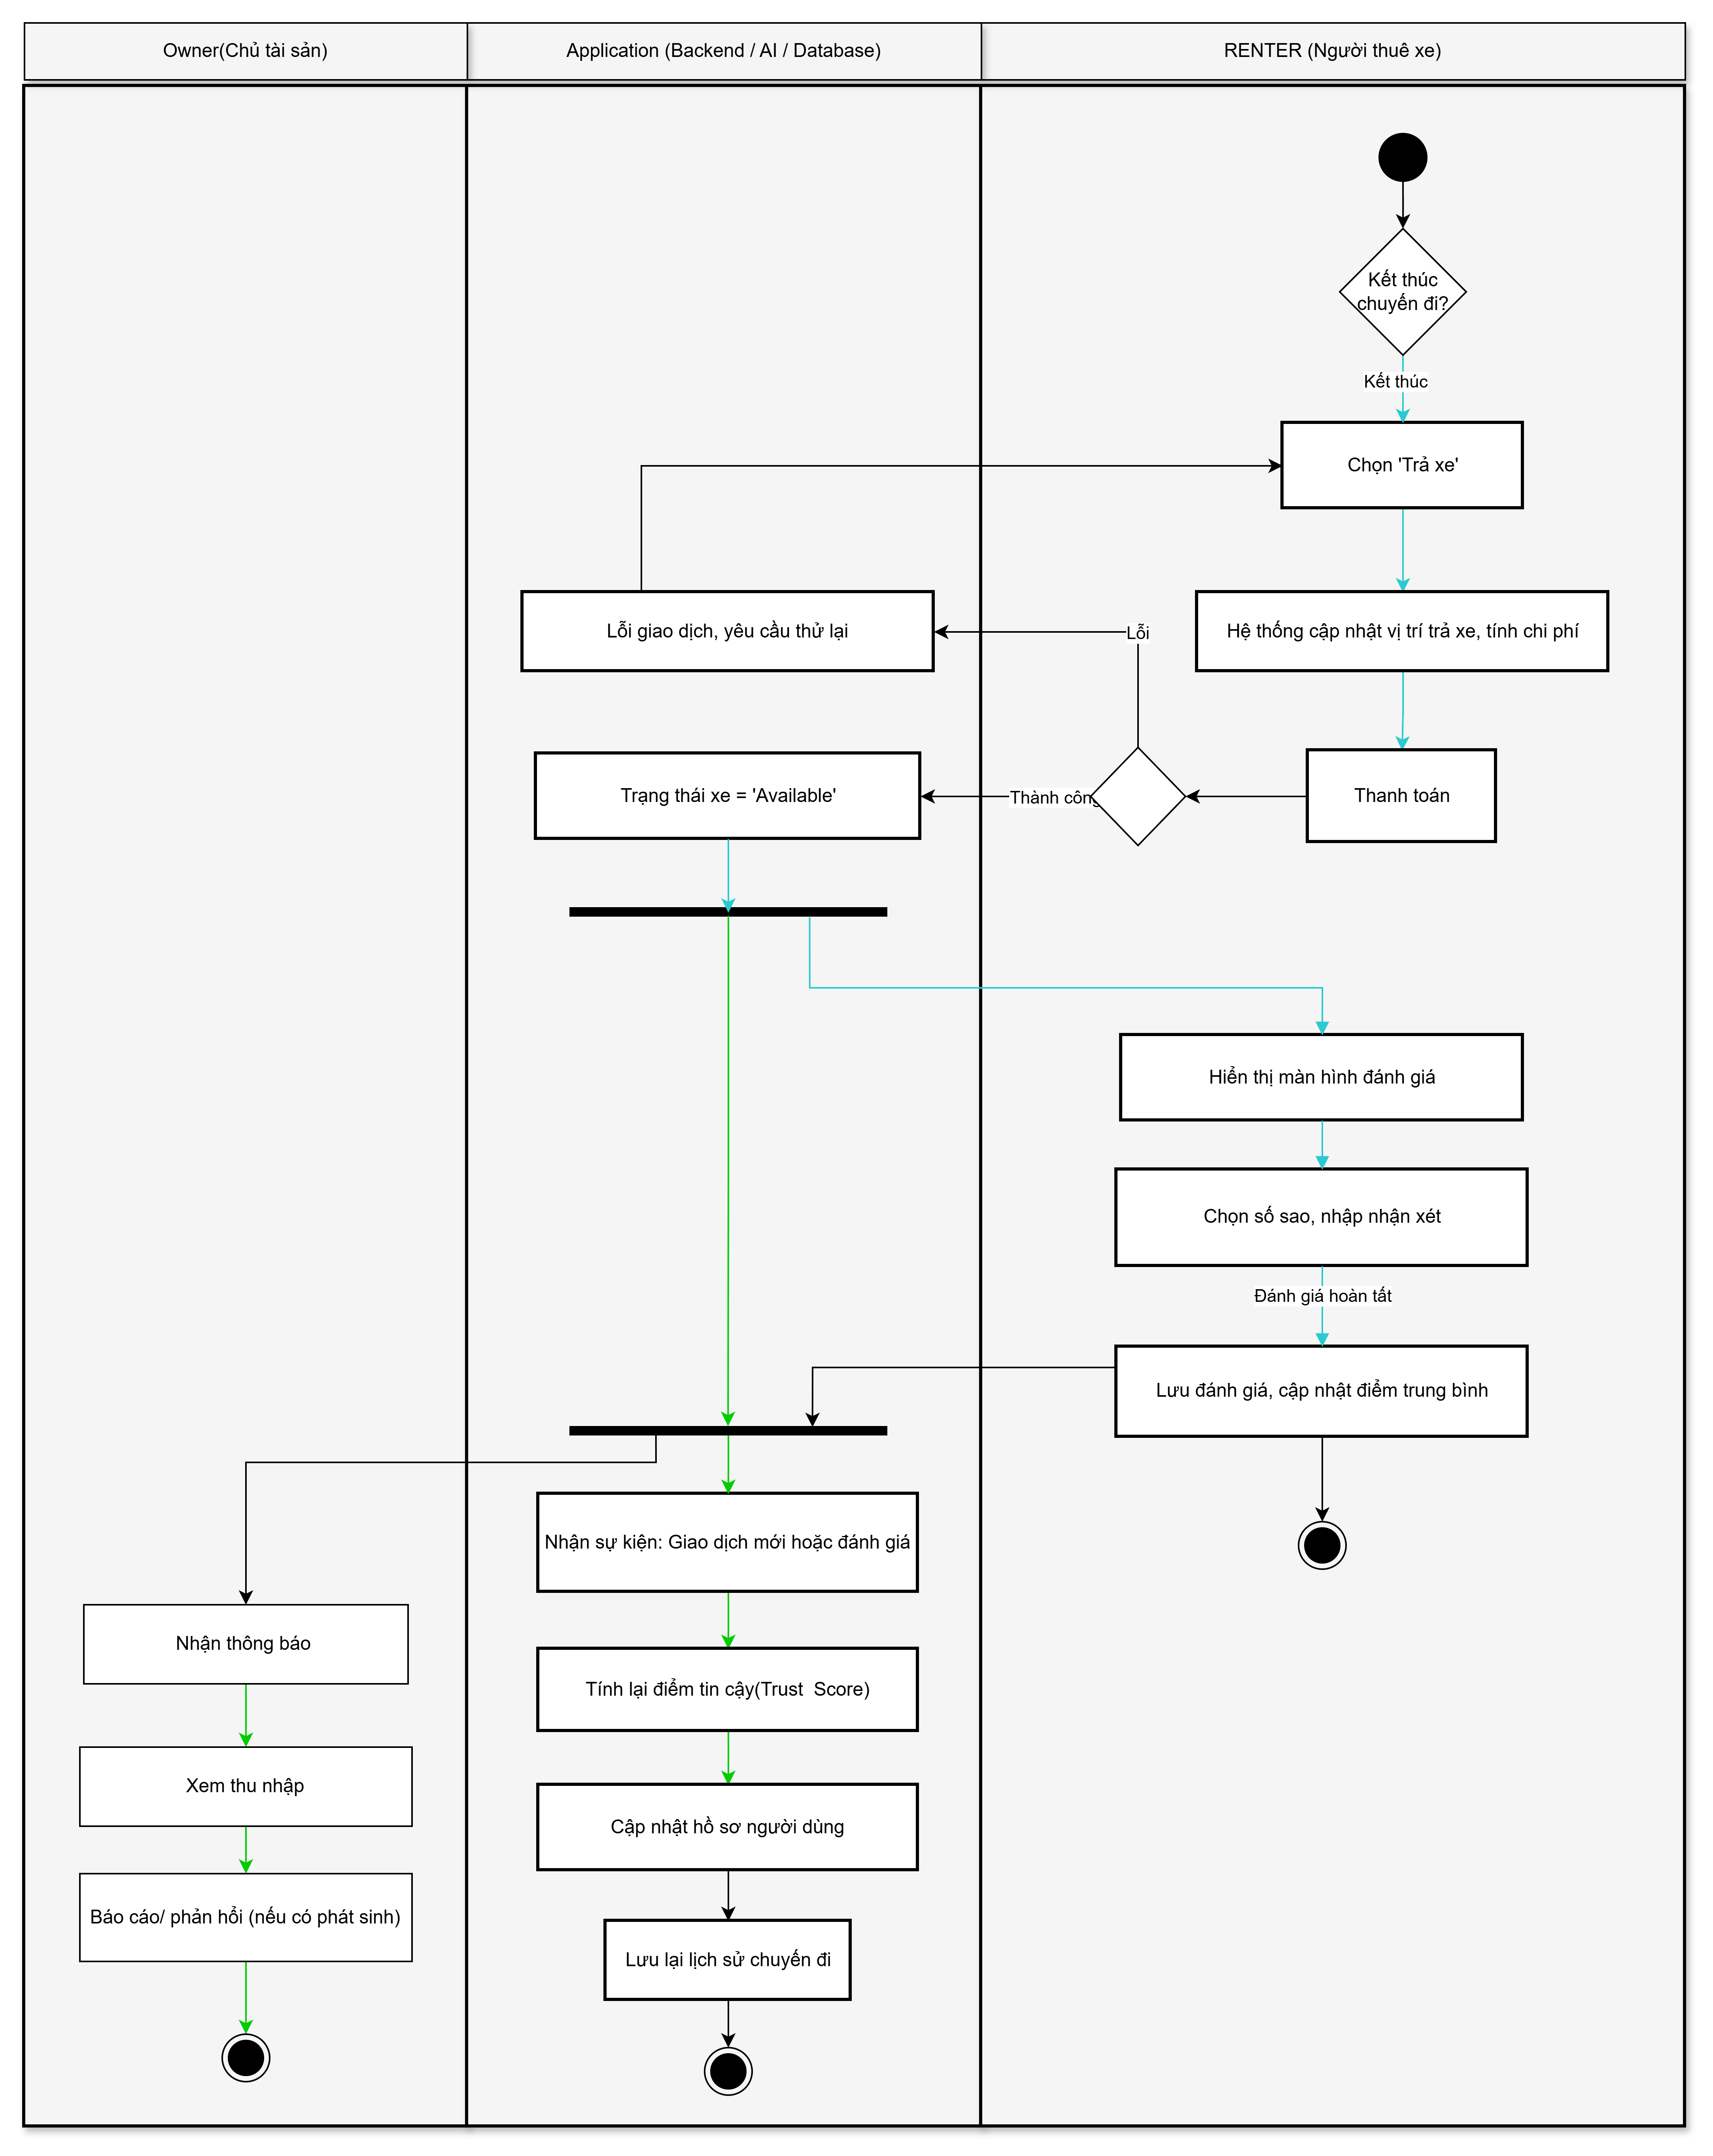
\includegraphics[width=1\textwidth]{Images/Activity/return.png}
    \caption{Returning Activity Diagram}
    \label{fig:return-activity}
\end{figure}

% ---------------------- REGISTER VEHICLE ----------------------
\subsubsection{Quy trình đăng ký xe cho thuê (UC-08)}
\label{subsec:regis-activity}
\small\textit{(Hình \ref{fig:regis-activity})}
\subsubsection*{Mục tiêu:}
Cho phép chủ xe thêm phương tiện của mình vào hệ thống để chia sẻ hoặc cho thuê, đảm bảo thông tin được xác thực và duyệt bởi quản trị viên trước khi hoạt động.
\subsubsection*{Actor chính: Chủ xe (Owner)}
\begin{figure}[H]
    \centering
    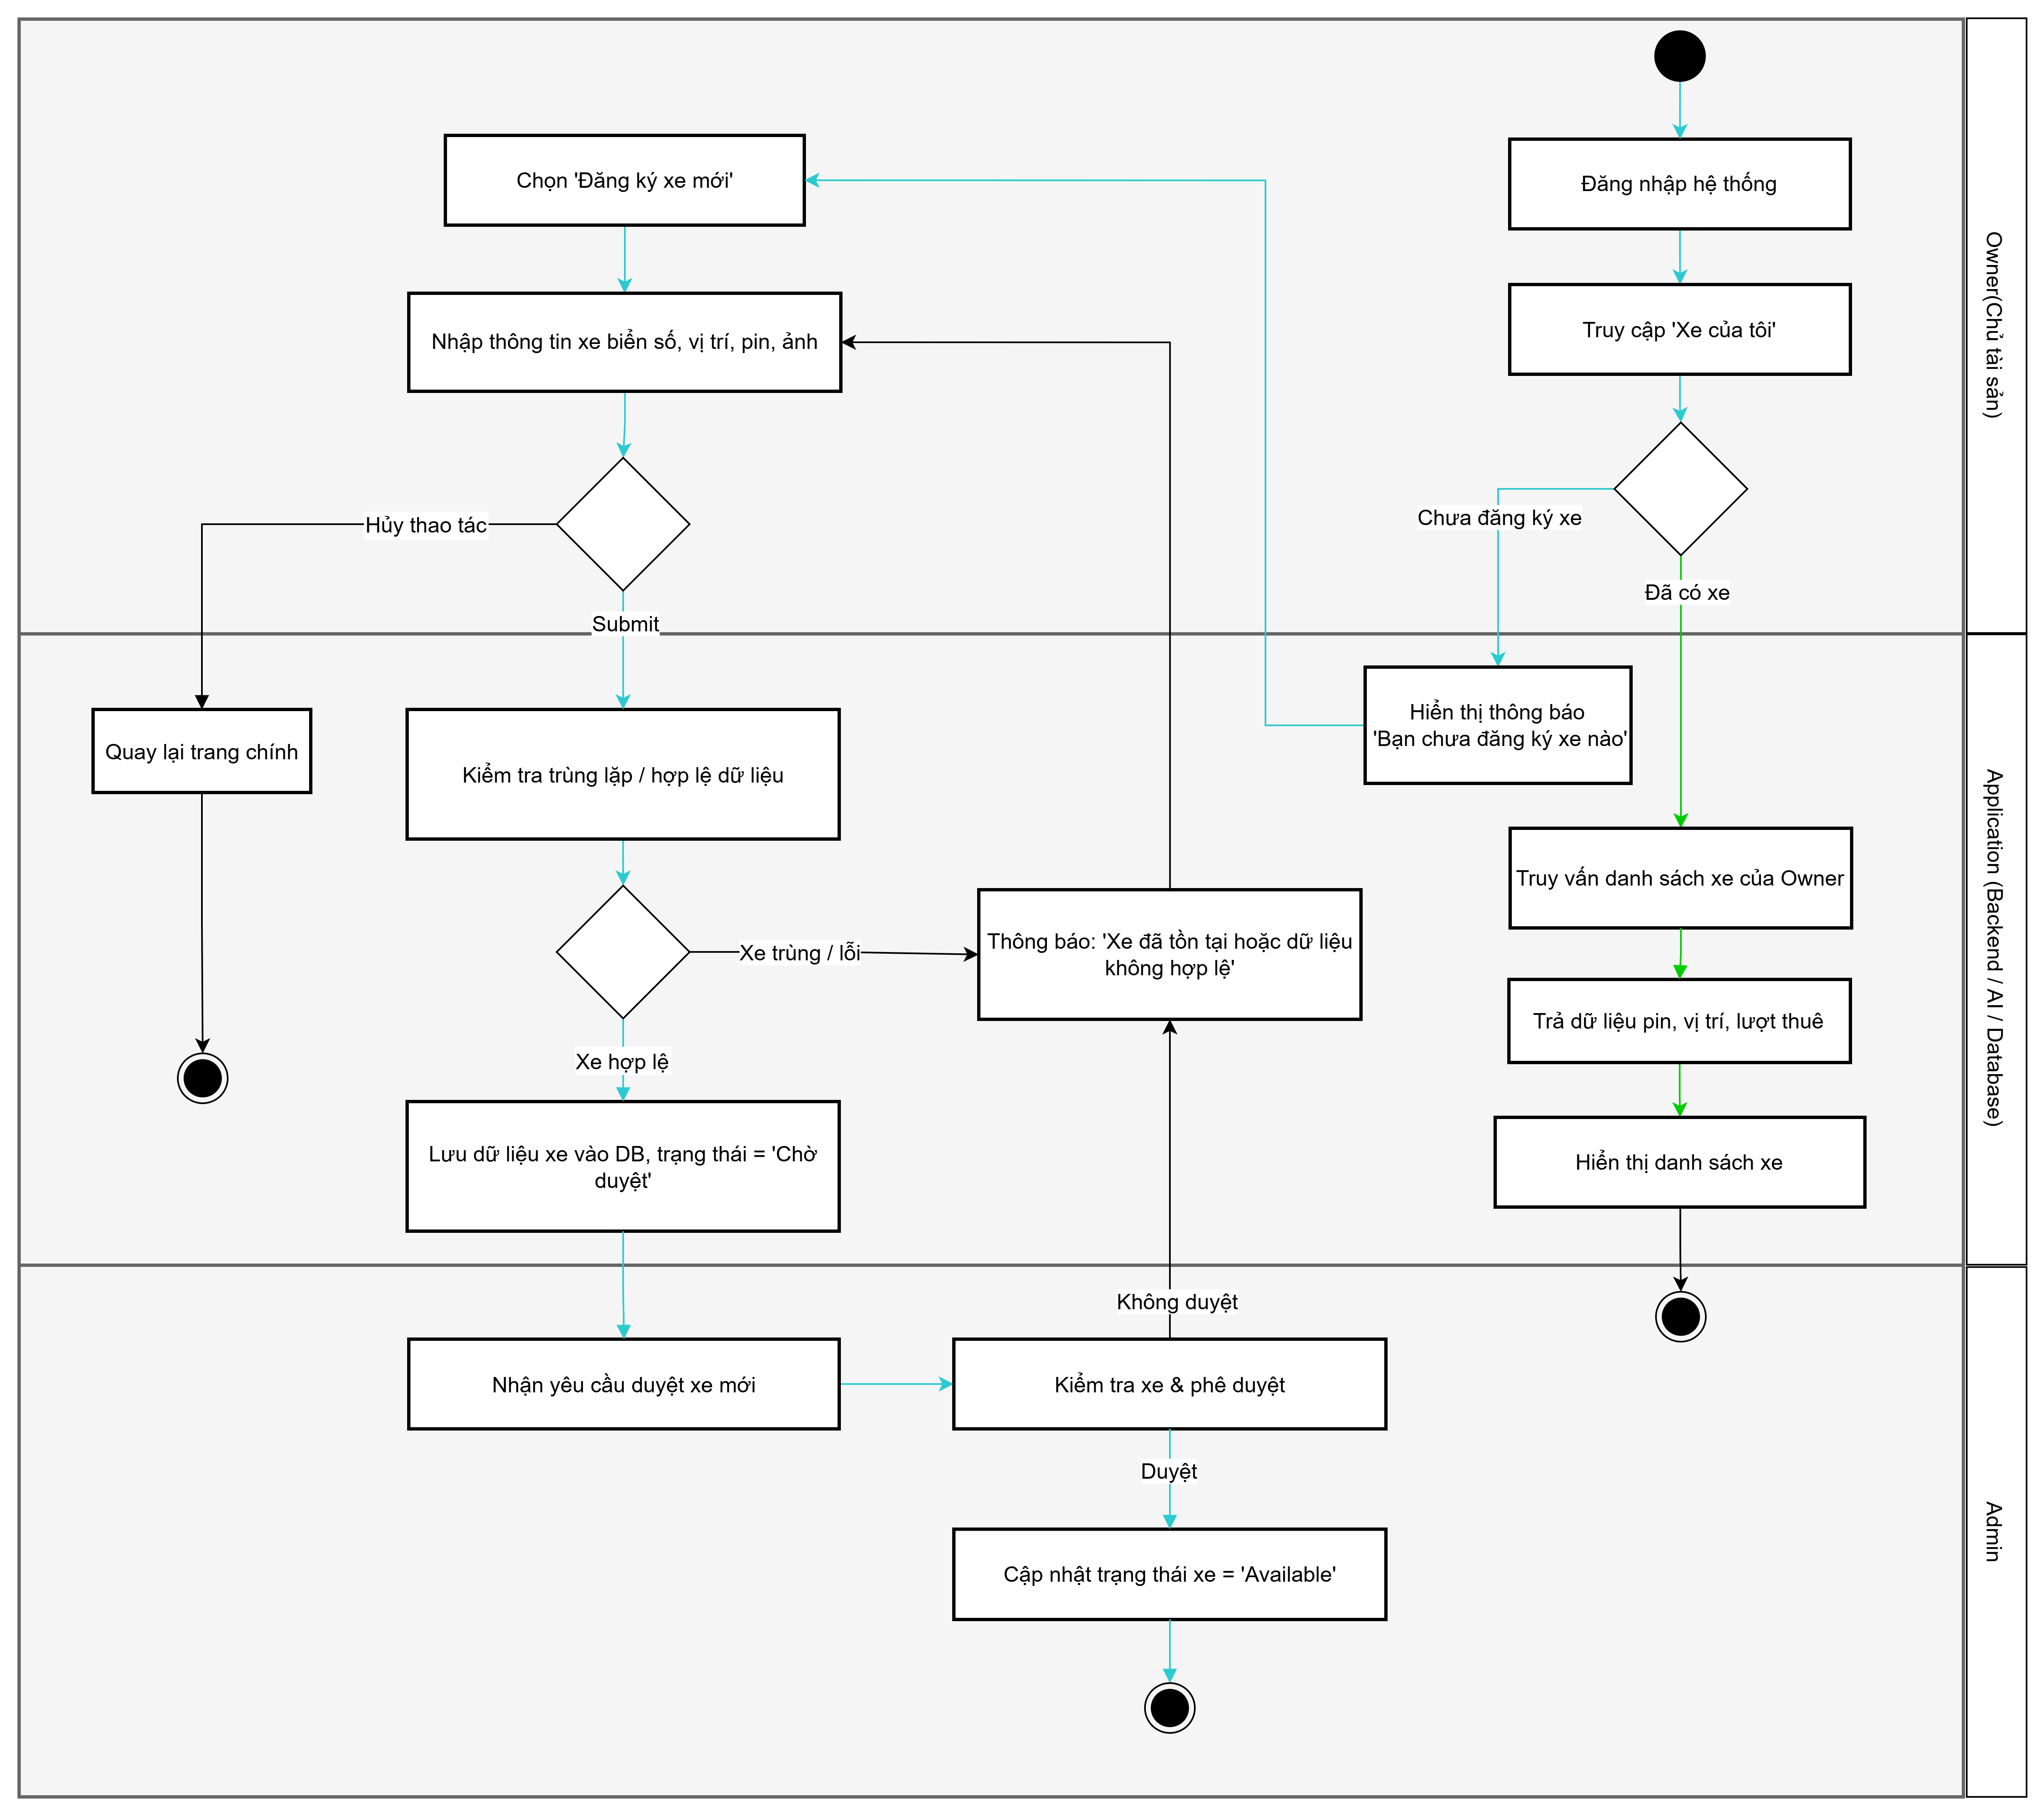
\includegraphics[width=1\textwidth]{Images/Activity/submit.png}
    \caption{Register Vehicle Activity Diagram}
    \label{fig:regis-activity}
\end{figure}
\subsubsection*{Các bước chính:}
1. Chủ xe đăng nhập và chọn chức năng “Đăng ký xe cho thuê”. \newline
2. Hệ thống hiển thị biểu mẫu để nhập thông tin xe: biển số, model, dung lượng pin, giá thuê, vị trí và hình ảnh. \newline
3. Chủ xe nhập thông tin và gửi yêu cầu đăng ký. \newline
4. Hệ thống kiểm tra dữ liệu hợp lệ (trùng biển số, định dạng ảnh, thông tin bắt buộc). \newline
5. Nếu hợp lệ, hệ thống tạo bản ghi xe mới trong cơ sở dữ liệu với trạng thái “Chờ duyệt (Pending)”. \newline
6. Gửi thông báo đến quản trị viên để xem xét và phê duyệt. \newline
7. Sau khi được duyệt, xe chuyển sang trạng thái “Available” và sẵn sàng cho thuê.
\subsubsection*{Luồng thay thế:}
- Chủ xe có thể lưu bản nháp nếu chưa hoàn tất thông tin. \newline
- Nếu phát hiện lỗi dữ liệu (trùng biển số, ảnh sai định dạng), hệ thống hiển thị thông báo để người dùng chỉnh sửa.

% ---------------------- MANAGE VEHICLE ----------------------
\begin{figure}[H]
    \centering
    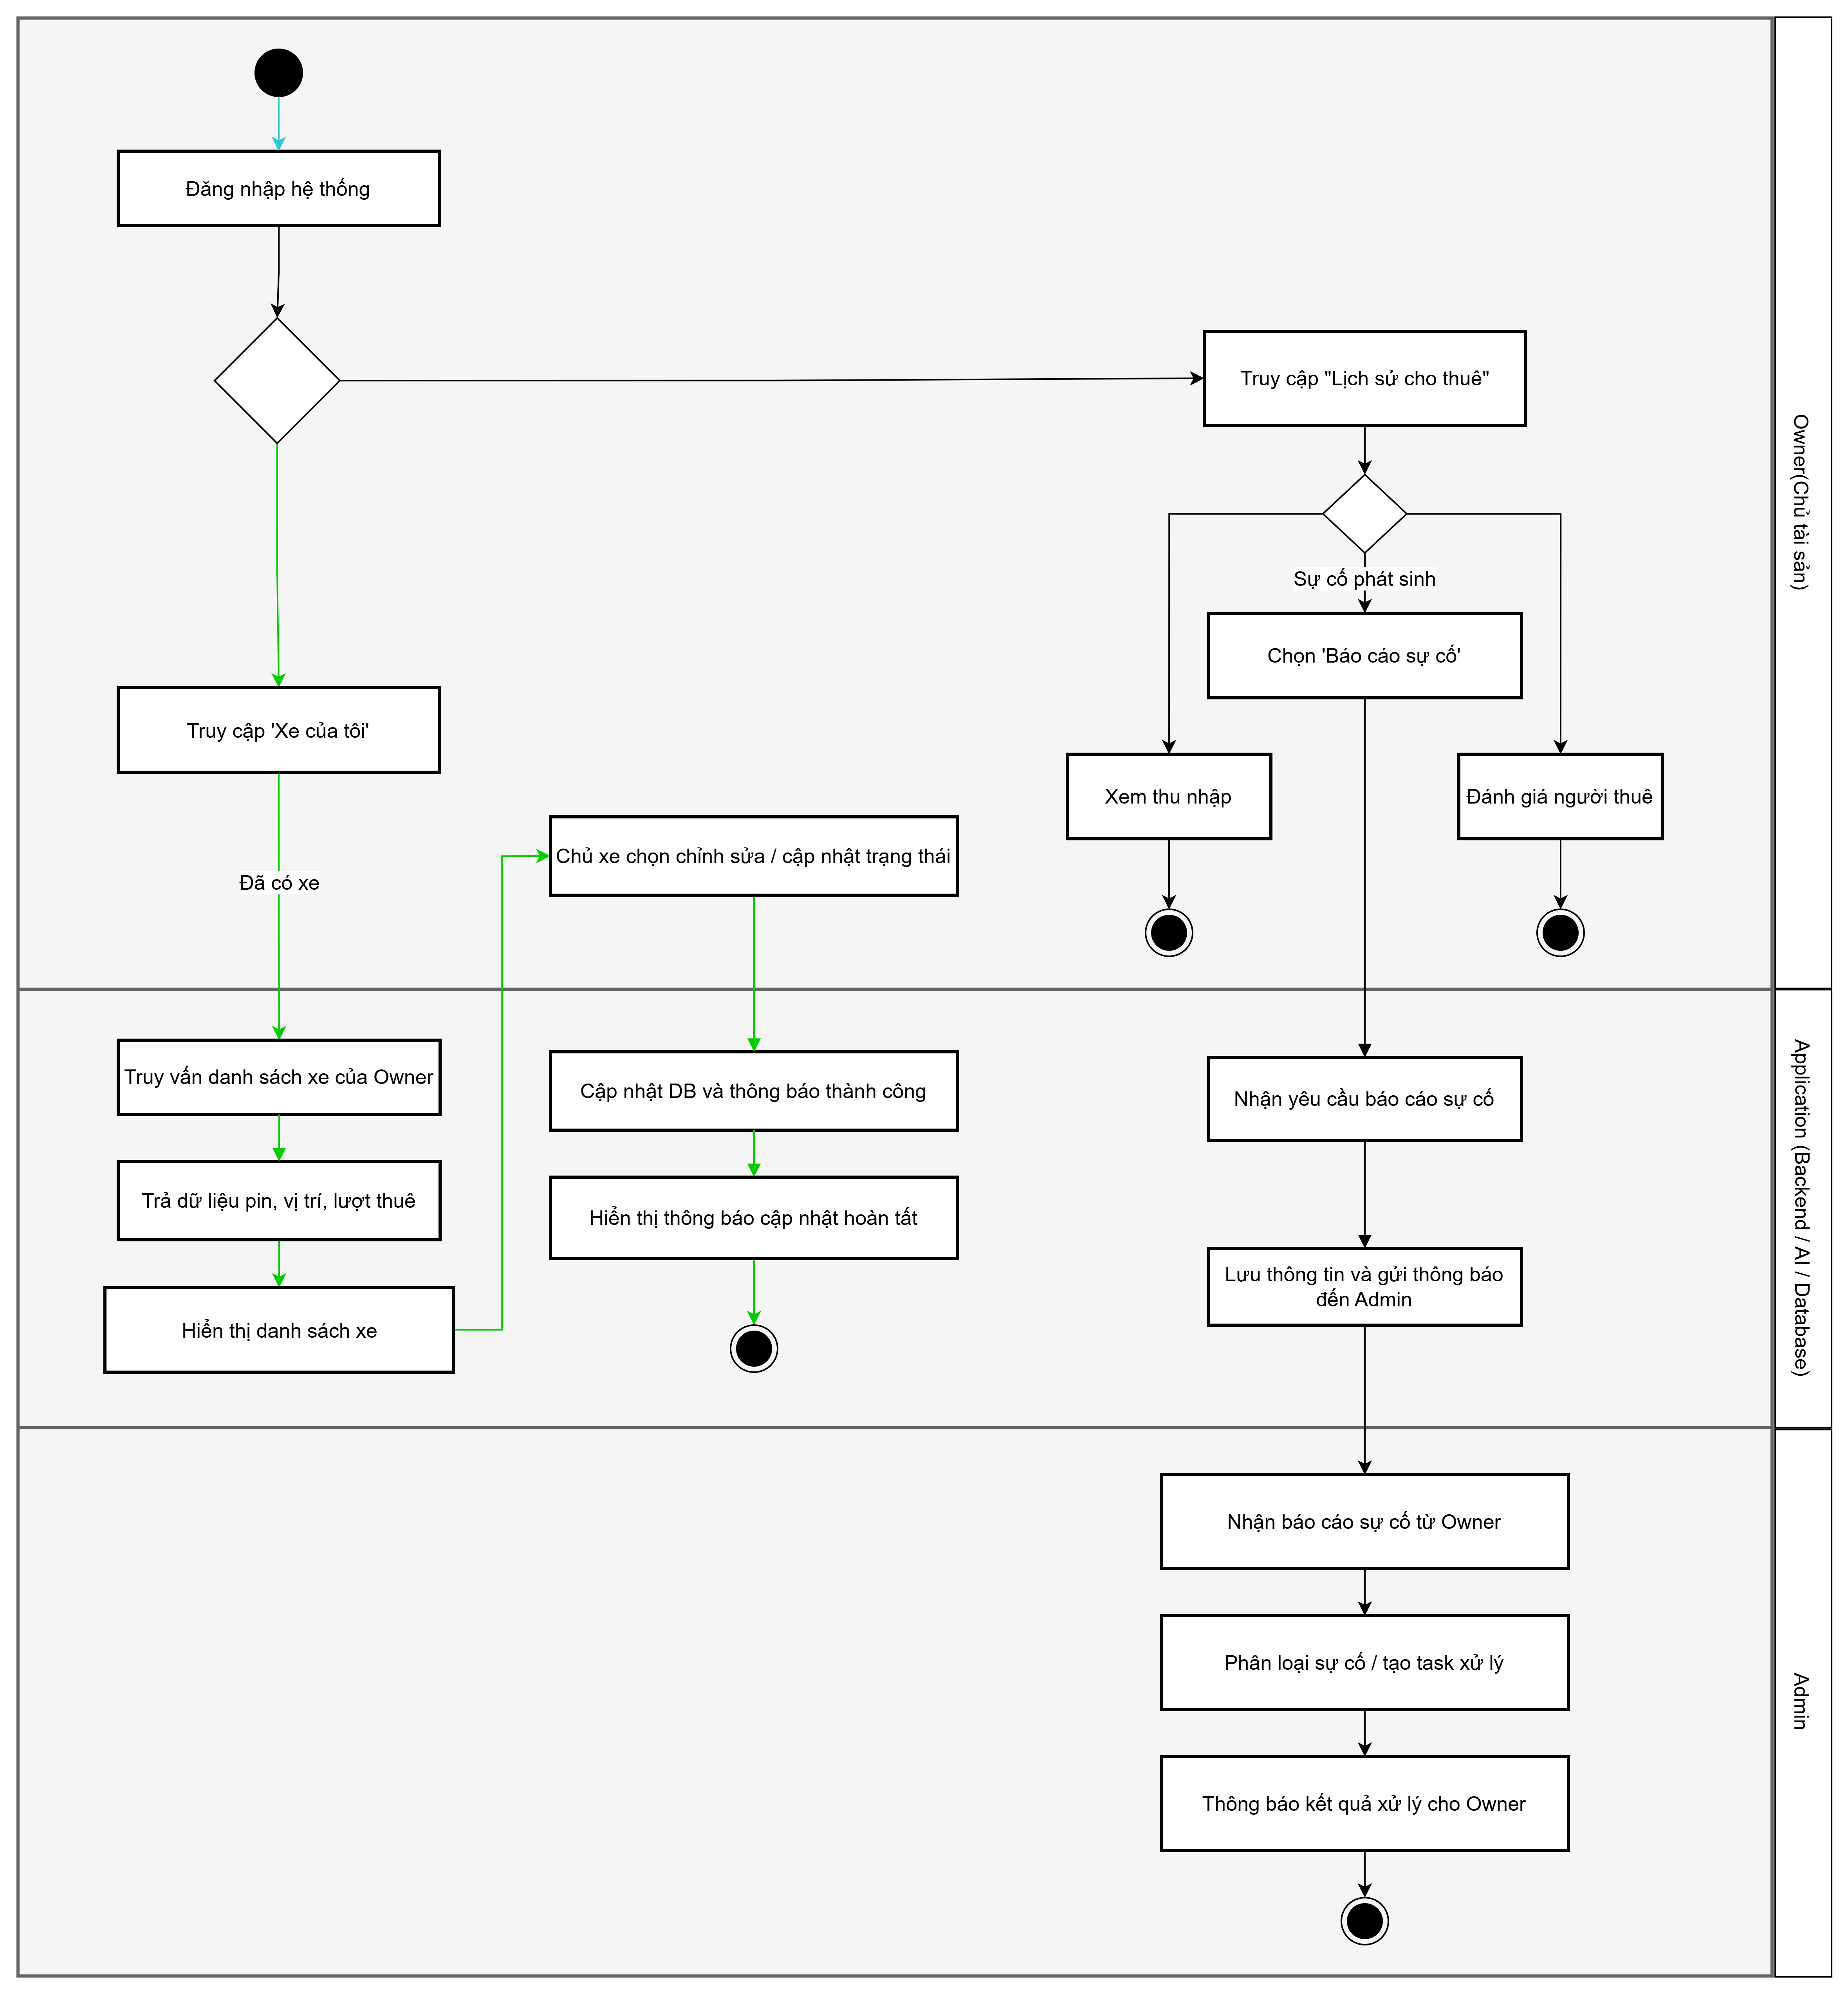
\includegraphics[width=1\textwidth]{Images/Activity/owner_management.png}
    \caption{Manage Vehicle Activity Diagram}
    \label{fig:manage-bike-activity}
\end{figure}
\subsubsection{Quy trình quản lý xe của chủ (UC-09)}
\label{subsec:manage-bike-activity}
\small\textit{(Hình \ref{fig:manage-bike-activity})}
\subsubsection*{Mục tiêu:}
Cho phép chủ xe theo dõi, cập nhật và quản lý các xe đã đăng ký cho thuê, đảm bảo thông tin xe luôn chính xác và đồng bộ với hệ thống.
\subsubsection*{Actor chính: Chủ xe (Owner)}
\subsubsection*{Các bước chính:}
1. Chủ xe đăng nhập và chọn mục “Quản lý xe”. \newline
2. Hệ thống hiển thị danh sách tất cả xe mà chủ xe đã đăng ký. \newline
3. Chủ xe chọn một xe để xem thông tin chi tiết. \newline
4. Thực hiện các thao tác: cập nhật giá, trạng thái pin, vị trí, hoặc tạm ẩn xe khỏi danh sách cho thuê. \newline
5. Hệ thống xác nhận và lưu thay đổi vào cơ sở dữ liệu. \newline
6. Các thay đổi được đồng bộ và phản ánh lên bản đồ xe cho thuê.
\subsubsection*{Luồng thay thế:}
- Chủ xe có thể kích hoạt cập nhật vị trí tự động qua GPS. \newline
- Xe đang cho thuê không thể bị ẩn hoặc xóa khỏi hệ thống cho đến khi kết thúc hành trình.

% ---------------------- ADMIN PROCESS ----------------------
\subsubsection{Quy trình quản trị hệ thống (UC-10, UC-11, UC-12)}
\label{subsec:admin-activity}
\small\textit{(Hình \ref{fig:admin-activity})}
\subsubsection*{Mục tiêu:}
Đảm bảo nền tảng hoạt động ổn định, an toàn và minh bạch thông qua việc kiểm duyệt xe, quản lý người dùng, và theo dõi hiệu quả hoạt động chung của hệ thống.
\subsubsection*{Actor chính: Quản trị viên (Admin)}
\subsubsection*{Các bước chính:}
1. Admin đăng nhập vào hệ thống quản trị. \newline
2. Hệ thống hiển thị bảng điều khiển (Dashboard) với các module: \textit{Duyệt xe}, \textit{Quản lý người dùng}, \textit{Báo cáo - Thống kê}. \newline
3. Admin chọn module cần thao tác:
3.1. \textbf{Duyệt xe:} Xem danh sách xe chờ duyệt, kiểm tra thông tin, hình ảnh, giấy tờ → phê duyệt hoặc từ chối → hệ thống cập nhật trạng thái và gửi thông báo cho chủ xe.\\
3.2. \textbf{Quản lý người dùng:} Xem danh sách người dùng, khóa/mở khóa tài khoản, thay đổi quyền truy cập (User, Owner, Admin), gửi cảnh cáo cho người vi phạm.\\
3.3. \textbf{Báo cáo - Thống kê:} Chọn loại báo cáo (doanh thu, lượt thuê, hoạt động theo khu vực), hệ thống tổng hợp dữ liệu, hiển thị biểu đồ và cho phép xuất file (PDF, Excel).\\
4. Sau khi hoàn tất thao tác, hệ thống lưu lại log quản trị (audit trail) để theo dõi thay đổi. \newline
5. Quản trị viên có thể đăng xuất hoặc chuyển sang module khác mà không ảnh hưởng dữ liệu.
\subsubsection*{Luồng thay thế:}
- Nếu dữ liệu bị lỗi hoặc chậm cập nhật, hệ thống hiển thị thông báo “Dữ liệu đang đồng bộ”. \newline
- Khi không đủ quyền thao tác, hiển thị cảnh báo “Không đủ quyền truy cập”. \newline
- Admin có thể lọc dữ liệu hoặc thay đổi thời gian xem thống kê linh hoạt.

% ---------------------- FIGURES ----------------------
\begin{figure}[H]
    \centering
    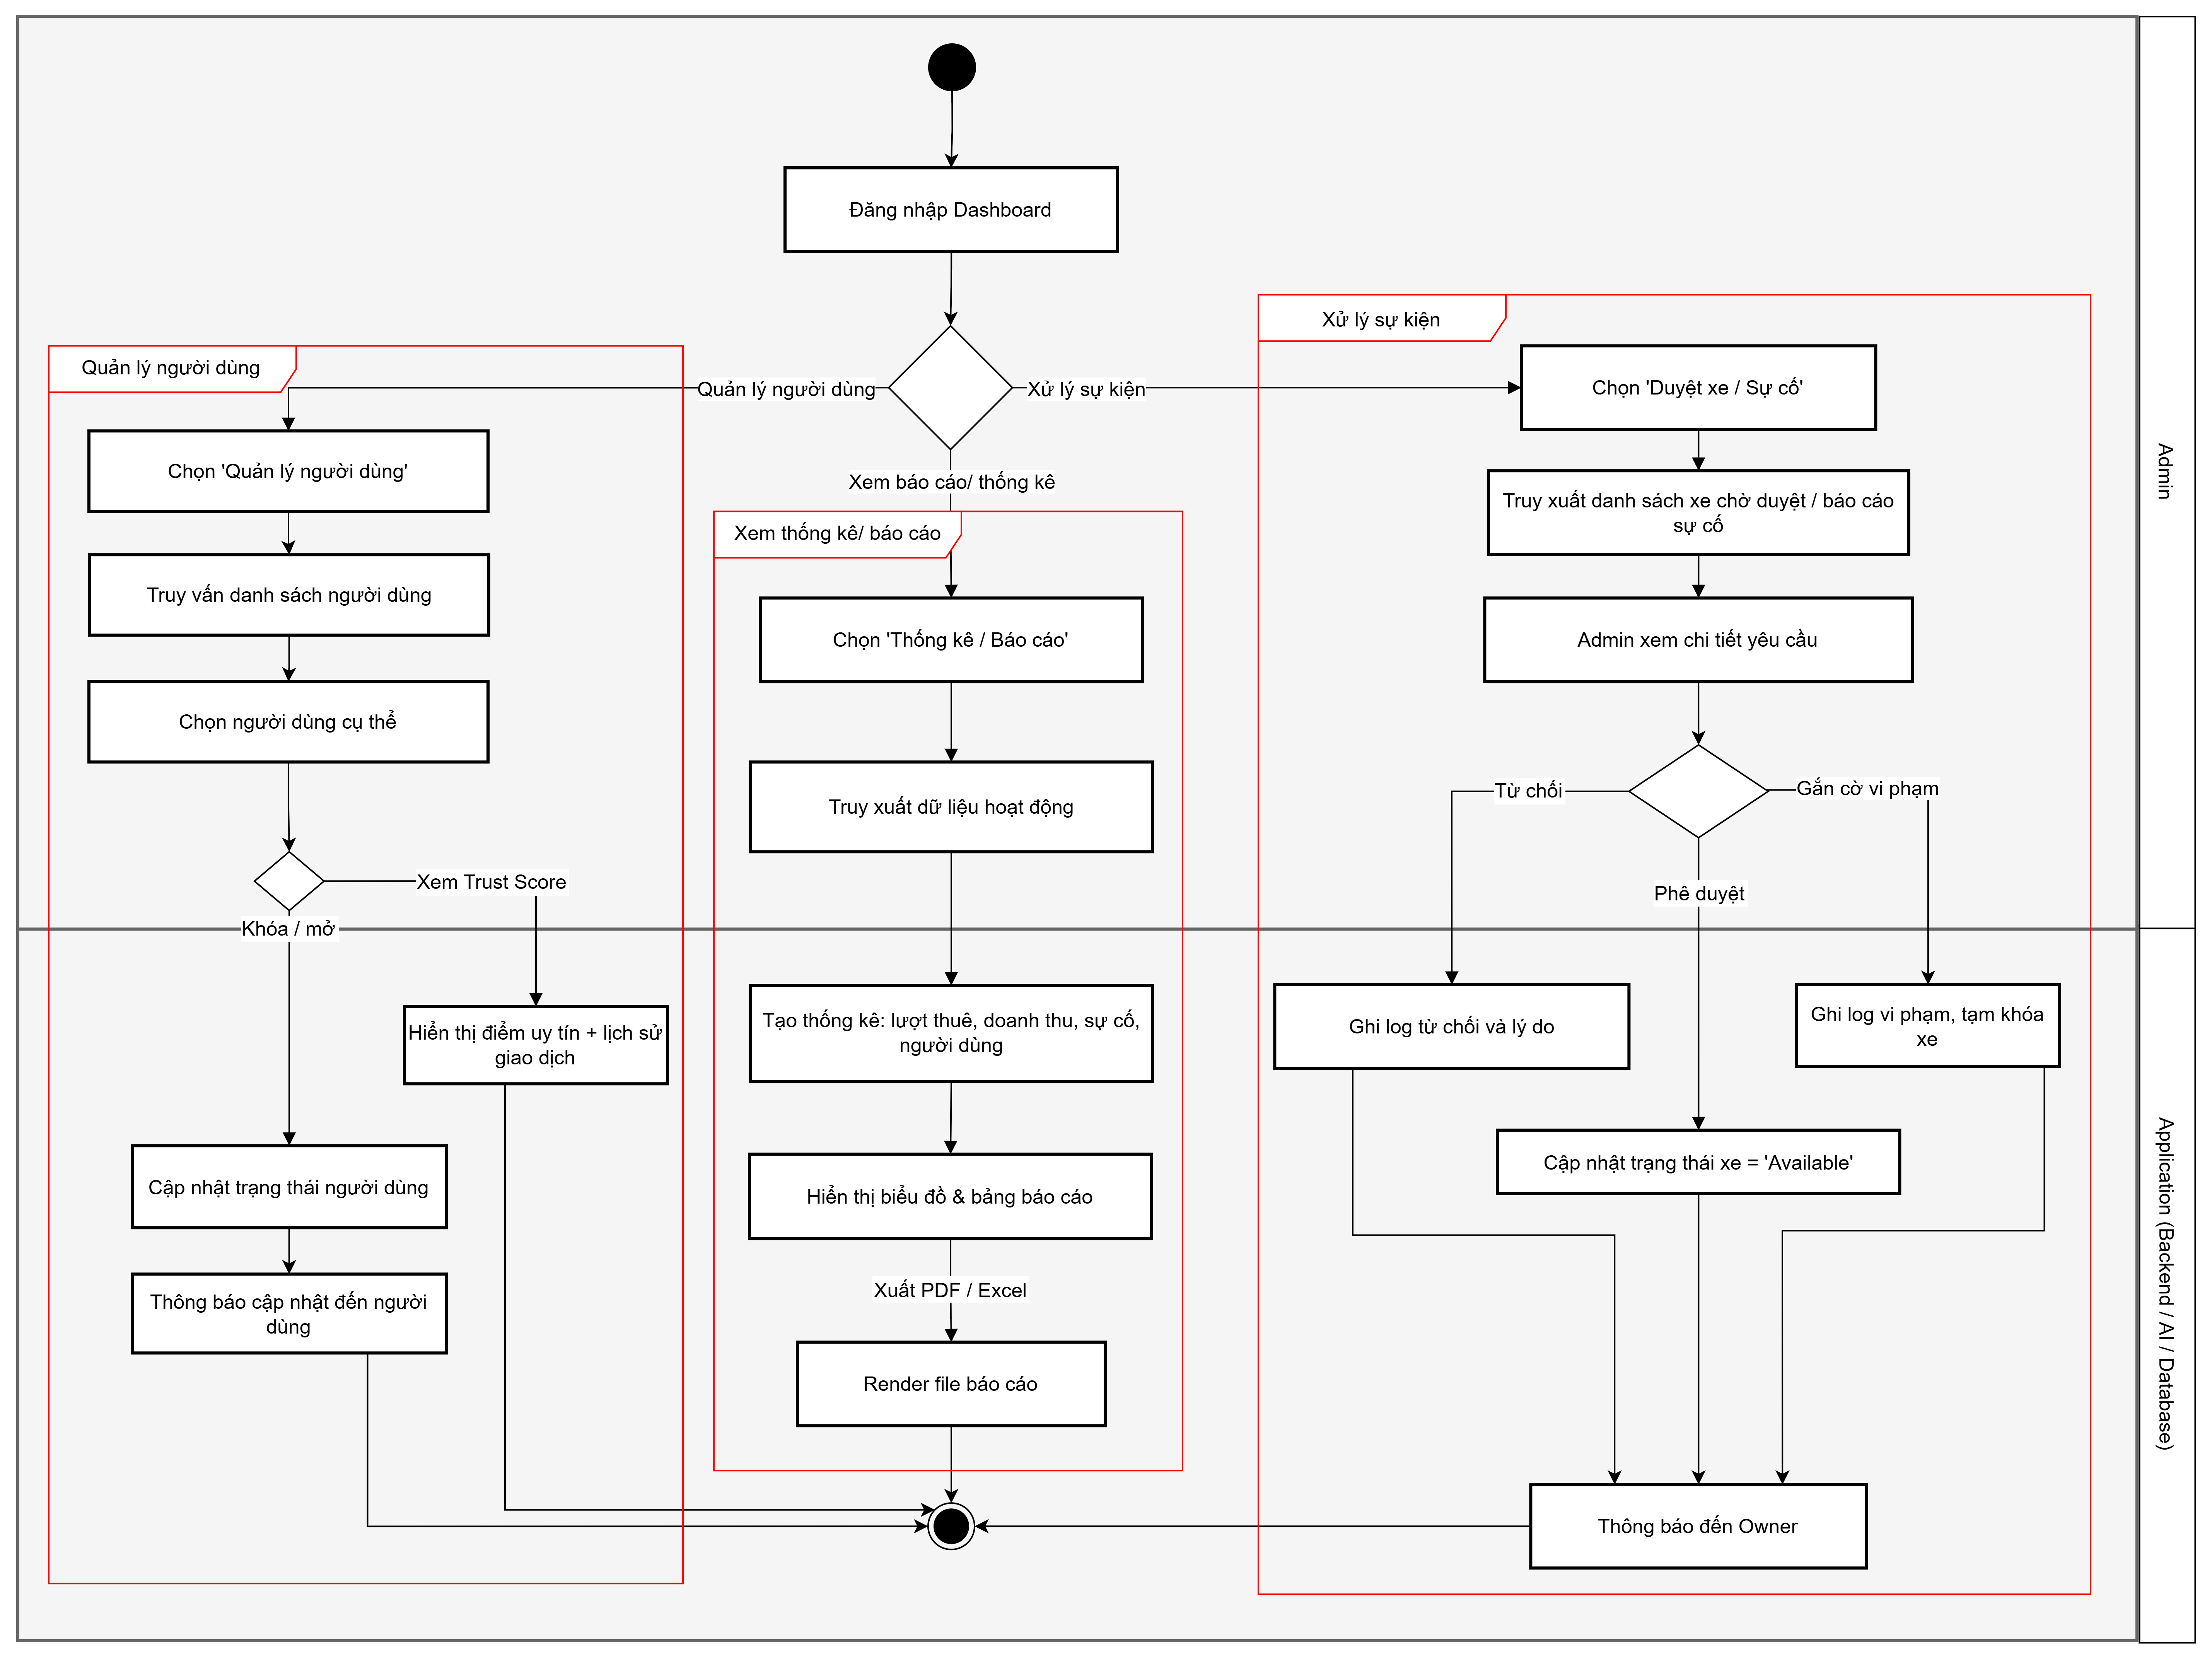
\includegraphics[width=1\textwidth]{Images/Activity/admin.png}
    \caption{Administrative Action Activity Diagram}
    \label{fig:admin-activity}
\end{figure}
